\section{Storage Architecture for Data-Intensive Computing}


\begin{figure}[ht]
    \centering
    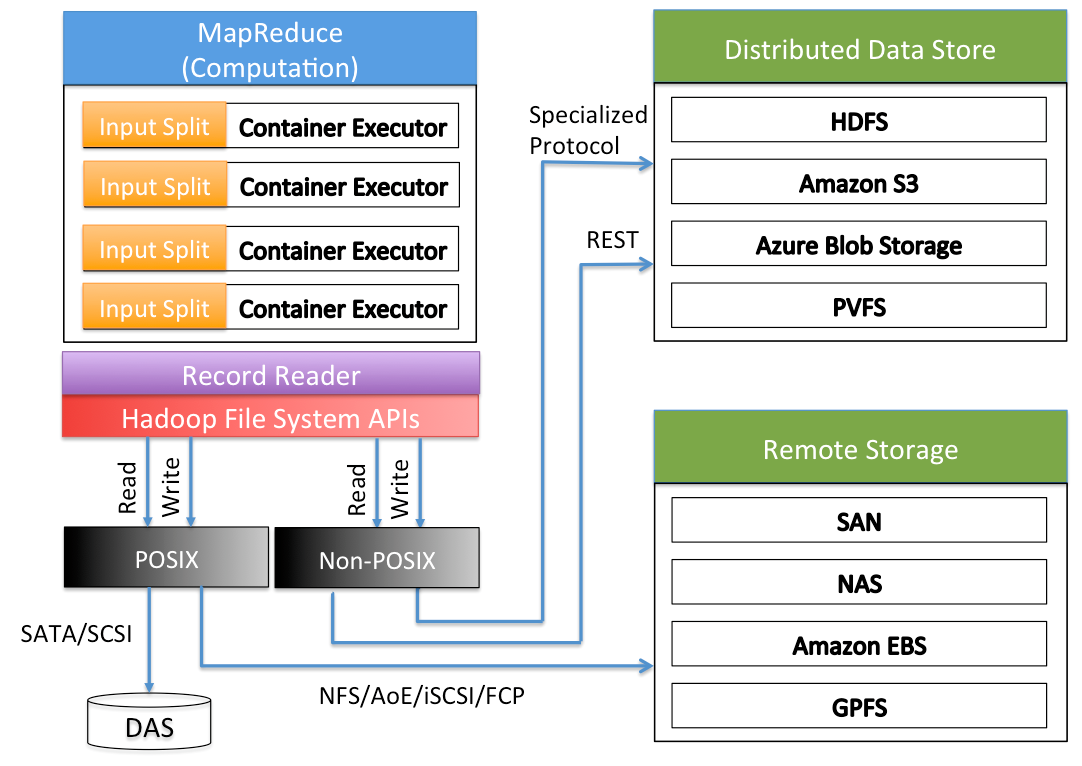
\includegraphics[width=0.8\textwidth]{figures/hadoop_model.png}
    \caption{System configuration of Hadoop.  Each slot handles one input split and uses the RecordReader object to read data from a POSIX compliant file system or a non-POSIX compliant file system, e.g. distributed data store.}
    \label{fig:hadoop_model}
\end{figure}

The most common way to deploy a Hadoop system is to configure a node to run both Hadoop MapReduce and Hadoop HDFS, which can avoid bringing data to computation.
However, data management, in many cases, requires separating computing and storage nodes for flexibility and efficiency.
For example, enterprises prefer silos in order to manage high-value data.
Amazon Elastic MapReduce primary uses Amazon S3 for its persistent data storage.
Moreover, many high performance files systems are considered to replace HDFS in order to support both MapReduce application and other workload.
As a result, different scenarios require different ways to deploy Hadoop.
As shown in Figure \ref{fig:hadoop_model}, we can define three major types of Hadoop configuration as follows.

Previous work compared the performance of Hadoop
integrated with different types of storage architecture~\cite{ShaferJ2010_PhD}.
The author found that in the \emph{split architecture},
in which compute and data nodes are not co-located,
Hadoop has a imbalance issue of accessing data.
This can lead to poor I/O performance.
In the following, we discussed the use cases that integrate Hadoop with separate storage.
After that, we describe scheduling methods for Hadoop and cluster that are related to our work.

\subsubsection*{Parallel File System}
Several research studies show their interests in replacing HDFS with other high performance storage systems.  
W. Tantisiriroj et al \cite{TantisirirojWittawat2011Duality} argues that parallel file systems can support diverse workloads and provides a better tradeoff between performance and reliability.
The authors proposed a PVFS shim layer to incorporate data layout of PVFS to achieve data locality.
Maltzahn \etal considered Ceph as a scalable alternative to HDFS~\cite{MaltzahnC2010_Ceph}.
The authors create a mapping layer which is similar to the PVFS one.
GPFS is a shared-disked file system developed by IBM, and widely adopted in supercomputers. 
R. Ananthanarayanan \etal from IBM Research modify data layout in GPFS, and
expose this information to Hadoop~\cite{AnanthanarayananR2009_CloudAnalytics}.
These are the attempts to replace HDFS.

\subsubsection*{Enterprise Storage}

Another research study analyzed the feasibility to use a very powerful storage node
to accommodate Hadoop~\cite{PorterG2010_SuperDataNodes}.
The study finds that Hadoop performance is dominated by the bandwidth
between computing and storage facilities.
Some argue that is is necessary to decouple compute and storage nodes 
n big data analytics
because enterprise IT often deploys \textit{silos}
to manage high-value data.
However, decoupled Hadoop model would incur high cost on data loading
from the back-end storage system to compute nodes.
MixApart includes the data-aware task scheduler, the task-aware data scheduler and a caching mechanism, to optimize Hadoop performance~\cite{MihailescuM2012_MixApart}.
It mainly focused on workloads that repeat regularly.

\subsubsection*{Cloud Storage}

Cloud storage typically refers to object storage hosted in cloud.
Amazon S3 and Azure Blob Storage are two examples.
Object storage manages data as objects.
Different from POSIX-compatible file systems,
RESTful API is a common way to access object storage.
Object storage is the primary data repository on the cloud.
Many data-intensive systems, \eg Amazon Elastic MapReduce and Azure HDInsight,
support using object storage as the back-end storage~\cite{aws, WindowsAzure}.
It is generally considered suboptimal than
the Hadoop reference architecture~\cite{hadoop}.

%\begin{table*}[h]
\caption{Comparisons of Hadoop models with different storage architecture}
\begin{center}
\resizebox{\textwidth}{!}{\begin{tabular}{| l | p{4.5cm} | p{4.5cm} | p{4.5cm} |}
\hline
 & \bf{Hadoop Reference Model} & \bf{Remote Storage Model} & \bf{Cloud Storage Model} \\
 \hline
Resource sharing & Dedicated Hadoop cluster & Enable time and space sharing & Same as the remote storage model \\
\hline
Deployment flexibility & The ratio between computation and storage resources remains fixed & Highly flexible to determine the size of computation and storage resource & Same as the remote storage model \\
\hline
Performance scalability & Scale-out easily & Proportional to storage I/O capability and network bandwidth & Network limitation \\
\hline
Read/Write Performance & Depends on local disk configuration & Support concurrent read/write (high I/O performance) & Long latency for REST and SOAP protocol \\
\hline
Replication & Triple replication is common & Block-level replication & Geo-replication is considered to reduce latency \\
\hline
Hadoop compatibility & Native support & Mounted as local storage, e.g. NFS & Only Amazon S3 is supported by default \\
\hline
Hadoop optimization & Schedulers are optimized for data locality & Not optimized & Not optimized \\
\hline
Extra & Hadoop is optimized for this model, but fails to apply to many use cases & Enterprise storage supports rich functions, e.g. de-duplication, archiving, data lifecycle management & Best fits the cloud computing scenario \\
\hline
\end{tabular}}
\end{center}
\label{tab:model_comparison}
\end{table*}
